\chapter{Implementacja modelu programowego}
%TODO Jak już opisze Pan na początku koncpecję to będzie to jasne. Tu trzeba się do tego odwołać. Bo w tej postaci to to wygląda tak, że sobie Pan to po prostu rozaważa... %ODP OK

Pierwszym etapem weryfikującym poprawność przedstawionej koncepcji było stworzenie modeli programowych algorytmów MeanShift oraz Hog+SVM, bez warstwy nadzorującej/sterującej dronem. 
Wybrano środowisko MATLAB ze względu na jego powszechne zastosowanie w branży naukowej/inżynierskiej, co skutkuje olbrzymią bazą bibliotek i materiałów pomocniczych. 
W tym przypadku MATLAB ułatwia pracę na obrazach lub sekwencjach wideo poprzez: wczytywanie materiału, wyświetlanie, dostęp do poszczególnych klatek oraz zapewnia wiele wbudowanych funkcji, m.in. do konwersji określonych przestrzeni barw oraz klasyfikacji z wykorzystaniem maszyny wektorów nośnych. %TODO może klasyfikacji z wykorzystaniem %ODP OK

\section{Model MeanShift}

Skrypt rozpoczyna działanie od wyznaczenia jądra obszaru o wymiarach $100 \times 100$ (zgodnie ze schematem \ref{fig:kernel_build}) oraz jego gradientów. %TODO tu by się przydały odnośniki do stosowanych wzorów.
Po tym następuje właściwa część algorytmu, która pracuje na wczytanym materiale wideo, przekonwertowanym do przestrzeni HSV. 
Obszarem śledzonym jest kwadrat $100\times 100$, który dla pierwszej klatki obrazu jest zlokalizowany w miejscu obecności śledzonego obiektu. %TODO co to jest miejsce startowe ??? %ODP OK
Dla tego fragmentu obliczany jest histogram barw. 
Następnie, dla kolejnych klatek, obliczany jest histogram kandydatów ostatecznie zestawiając go z oryginalnym i wyznaczając przesunięcie w pionie i poziomie. %TODO styl. Następnie, dla kolenych klatek, obliczane.... %ODP OK
Dla każdej z klatek operacja ta jest przeprowadzana 10 razy, poprawiając precyzję ostatecznego przesunięcia. 
Przed rozpoczęciem przetwarzania kolejnej klatki, następuje aktualizacja pozycji śledzonego obszaru. %TODO Obszaru ? %ODP OK
Po wykonaniu algorytmu dla zdefiniowanej liczbie klatek, skrypt wyświetla film w oryginalnych barwach RGB z dorysowaną czerwoną ramką otaczającą śledzony obszar, co pozwala wizualnie sprawdzić poprawność działania całego kodu. 
Niestety, czas wykonania tej symulacji jest nieporównywalnie dłuższy od rzeczywistego trwania sekwencji i, przykładowo, na komputerze wyposażonym w procesor klasy i7 materiał o długości 685 klatek (ok. 11 sekund filmu) jest przetwarzany w czasie ok. 100 sekund.

Rysunek \ref{fig:meanshift_prog} przedstawia śledzenie obiektu w postaci czerwonej koszulki z ciemnym poziomym paskiem. Kolejne zrzuty są realizowane z odstępem 100 klatek. Zauważyć można poprawne działanie algorytmu nawet pomimo zmiany odległości obiektu od kamery.
 
\begin{figure}[]
	\centering
	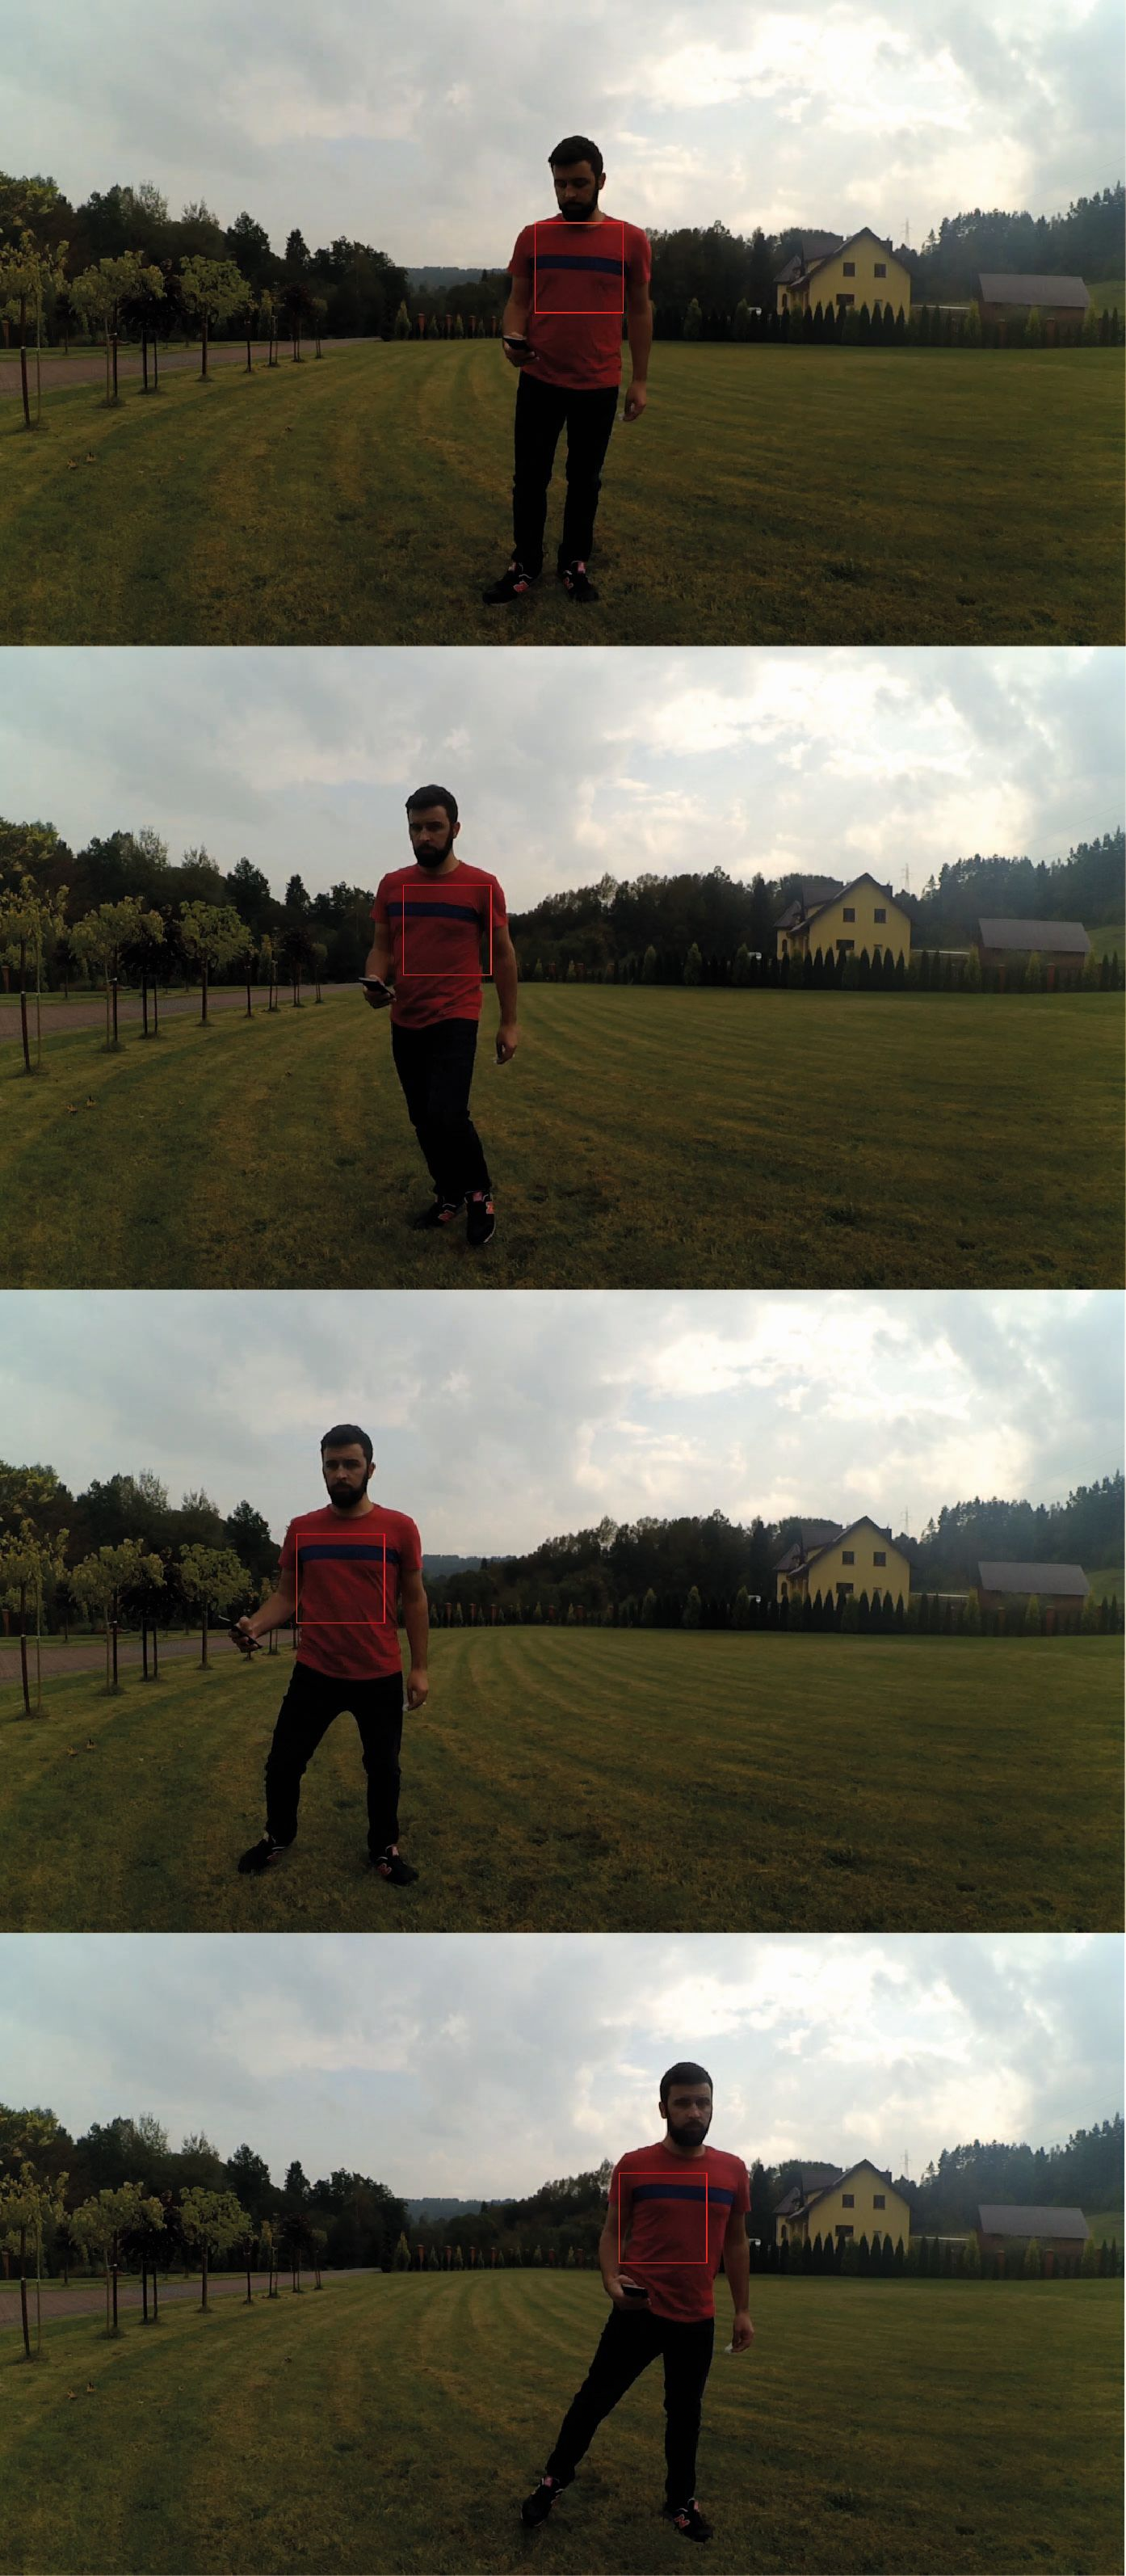
\includegraphics[width=16cm]{3_meanshift.jpg}
	\caption{Śledzenie MeanShift}
	\label{fig:meanshift_prog}
\end{figure}

%TODO 1. Obarzki mniejsze, a za to prostokąt wyraźniejszy. %ODP OK
%TODO 2. Jakieś inny test %ODP dodano w tej samej grafice
%TODO 3. Komentarz nt. działania algorymtu.

\section{Model HoG+SVM}


Głównym zadaniem modelu programowego jest próba detekcji osoby w przeskalowanym obrazie, w oparciu o obszar zainteresowań $144 \times 96$, którego środek stanowi punkt wybrany przez użytkownika. Podstawowym zadaniem jest jednak proces uczenia klasyfikatora SVM, który zostanie użyty nie tylko w modelu programowym, ale również w trakcie implementacji sprzętowej. %TODO Niejasne %ODP OK

\subsection{Uczenie}
Uczenie jest dość złożonym obliczeniowo procesem przetworzenia obrazów i ekstrakcji wektorów cech, na podstawie których powstanie płaszczyzna rozdzielająca próbki pozytywne od negatywnych. %TODO to żmudny to nie pasuje styl. %ODP OK
Przejście przez tak wielką liczbę obrazów ma charakter jednorazowy, po którym będzie dysponować się parametrami umożliwiającymi klasyfikację. 
Z tego względu nie zdecydowano się na implementację modułu uczącego w układzie FPGA -- tak ze względu na złożoność tego etapu, czas trwania procedury, jak i prawdopodobnie duży udział modułu w zużyciu zasobów logiki. 

Wybór padł na środowisko MATLAB dysponujące funkcjami wspierającymi metodę SVM. 
Skrypt korzysta z plików tekstowych zawierających listy próbek do wczytania, które ostatecznie muszą być w rozmiarze $128\times 64$. 
Wymiary próbek negatywnych mocno odbiegają od założonego wymiaru klasyfikowanego obrazu ($128\times 64$). 
Zdecydowano, iż w ich przypadku uczeniu poddany będzie obszar o wymiarach $128\times 64$ wycięty ze środka oryginałów. %TODO dlaczego raz jest 128x64 a kiedy indziej w $$. %ODP OK, nie wypatrzyłem tego. 
Proces tworzenia wektorów cech przeprowadzono zgodnie z informacjami zawartymi w rozdziale \ref{sec:HOG&SVM}; za normę blokową obrano L2 (\eqref{eq:HOG_norm3}).
Na bazie tak przygotowanych próbek powstaje tablica deskryptorów oraz druga, która przechowuje odpowiadające im wartości klas (1 lub 0). 
Z obu tablic korzysta dostępna w pakiecie Matlab funkcja \textit{svmtrain}, która zwraca strukturę \textit{svm\char`_struct} ze współczynnikami wykorzystywanymi w klasyfikacji. %TODO czego ? %ODP OK
Z kolei funkcja \textit{svmclassify} służy do klasyfikacji obrazu (a właściwie jego deskryptora). %TODO "w stanie" styl, personifikacja %ODP OK
Funkcję tę użyto w procesie testowania niezależnego zestawu danych złożonego z poprawnie sklasyfikowanych obrazów, by sprawdzić skuteczność klasyfikacji wyuczonego SVM. %TODO niejasne... raczej suteczność klasyfikiacji wyuczonego SVM. %ODP OK
Etap testowania jest dodatkowo przydatny -- pozwala na bazie eksperymentów zdefiniować optymalny rozmiar komórki (kwadratu pikseli), na bazie których liczony jest pojedynczy histogram. 
Tabela \ref{tab:HOG_cell_size} prezentuje wyniki, wśród których uwzględniony jest błąd, liczony jako stosunek liczby niepoprawnych klasyfikacji (0 zamiast i 1 zamiast 0) do liczby testowanych obrazów.
Eksperyment przeprowadzono na komputerze wyposażonym w procesor Intela klasy i7, trzeciej generacji.
\newcolumntype{P}[1]{>{\centering\arraybackslash}p{#1}}
\begin{table}[h]
	\centering
	\captionsetup{justification=centering,margin=1cm}
	
	\begin{tabular}{|P{3cm} |P{3cm} |P{4.5cm}| P{3.5cm}|}	
		\hline
		\rowcolor{lightgray} Rozmiar komórki [px] & Liczba elementów wektora cech & Błąd klasyfikacji [\%]  & Czas trwania obliczeń [s] \\ 
		\lbrack$2\times $2\rbrack			& 70308		& 3.4069		& 52min 42s		\\ 
		\hline		
		\lbrack$4\times 4$\rbrack			& 16740 	& 2.3344		& 14min 08s		\\ 
		\hline
		\lbrack$8\times 8$\rbrack			& 3780		& 3.3438		& 05min 01s		\\ 
		\hline
		\lbrack$16\times 16$\rbrack			& 756		& 5.1735		& 02min 50s		\\ 
		\hline
	\end{tabular}
	
	\caption{Skuteczność algorytmu na zbiorze testowym w zależności od wielkości pojedynczej komórki}
	\label{tab:HOG_cell_size}
\end{table}
%TODO czas trwania obliczeń. %ODP OK
%TODO jak jest liczony bład %ODP OK, nad tabelą

Okazuje się, że algorytm wykazuje największą skuteczność dla komórek o rozmiarze $4\times 4$. 
Zdecydowano się zatem na implementację algorytmu HOG w układzie FPGA właśnie dla tej wartości parametru. 
Szybkie obliczenia pokazują, że dla obrazu o wymiarach $128\times 64$ powstanie $32\times 16$ komórek, a idąc dalej, $31\times 15$ bloków po 4 histogramy po 9 wartości -- długość wektora cech będzie wynosić 16740. 
Oznacza to również, że po zakończonym procesie uczenia powstanie wektor współczynników o takiej długości. %TODO no chybo nie do końca, bo normalizacja w blokach zwiększa ten rozmiar. %ODP Mógłby Pan Doktor wyjaśnić? Ja po prostu dzielę 36 wartości danego bloku przez ich sumę+'1'. Więc wyjściem jest nadal 36 elementów na blok.

%TODO To co jest od "Uczenie" do tego momentu przenieść i zintegrować z opisem \section{Model HoG+SVM} %ODP OK


%TODO proszę to jednak podzielić osobno na uczenie i rozpoznawanie. %ODP OK

%Działanie skryptu rozpoczyna się od przeprowadzenia uczenia klasyfikatora, która bazuje na dwóch tablicach: jedna agreguje wektory cech, a druga przechowuje skojarzone z nimi klasy (0 lub 1). 
%Wykorzystywana baza obrazów wyposażona jest w pliki z ich listami (osobno dla pozytywnych i negatywnych przykładów), co umożliwia proste wczytywanie kolejnych próbek. 
%Oczekuje się tu rozmiaru $128\times 64$ pikseli, jednak niektóre (zwłaszcza negatywne) obrazy są za duże -- przeprowadza się tutaj wycięcie fragmentu o podanym wyżej rozmiarze ze środka każdej próbki. Kolejnymi etapami dla takiego obszaru są kolejno: konwersja do odcieni szarości oraz obliczenie wektora cech. 
 %TODO styl. potrzeby.. niepotrzebnie %ODP OK

\subsection{Rozpoznawanie}
Po uzyskaniu struktury ze współczynnikami można podjąć się klasyfikacji obszarów z obrazów wczytanych przez użytkownika.

Napisany w tym celu skrypt rozpoczyna działanie od wczytania obrazu wejściowego. 
Po zdefiniowaniu punktu będącego środkiem obszaru zainteresowań następuje realizacja algorytmu HOG+SVM dla każdej z 5 zdefiniowanych wcześniej skal.
Pierwszym krokiem jest obliczenie $5\times 9$ wektorów cech na fragmencie $144 \times 96$ -- celem jest znalezienie jak najlepszego wyniku detekcji.  %TODO niejasne, i styl z "planu".  %ODP OK
%TODO Czy to jest tylko w jednej skali licznone ? %ODP Nie, dla wielu - wyświetlany jest najlepszy wynik - wyświetlanie wszystkich wyników poniżej 0 wygląda dość nieczytelnie
Idąc za przykładem wbudowanej w MATLAB funkcji \textit{svmclassify}, następuje klasyfikacja każdego obliczonego wektora cech. Proces ten jest powtarzany dla każdej z wcześniej określonych skal. 
Końcowym etapem jest wyświetlenie oryginalnego obrazu w kolorze, z naniesionymi konturami: obszarów zainteresowań $144\times 96$, oraz pozytywnych detekcji o wymiarach $128\times 64$ -- przeskalowanych do rzeczywistego rozmiaru. Finalna detekcja jest obliczana na podstawie najlepszego (najniższego) wyniku klasyfikacji z zebranych wyników analiz wszystkich skal.

Przykłady detekcji w pojedynczych skalach zaprezentowano na rysunkach \ref{fig:SVMmodel}, \ref{fig:SVMmodel_2_5} oraz \ref{fig:SVMmodel_3}.
Różowym konturem oznaczono okno detekcji $144 \times 96$, natomiast na czerwono zakreślono ostateczne obszary $128\times 64$ pozytywnie wybrane przez klasyfikator. Przedstawiono również tabele z wynikami klasyfikacji poszczególnych deskryptorów. Pogrubione zostały pozytywne wyniki detekcji.%TODO ale trzeba napisać co to za wyniki. %ODP OK
\begin{figure}[]
	\centering
	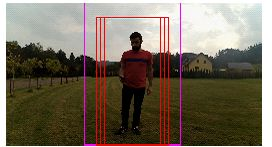
\includegraphics[width=10cm]{3_SVM_model.jpg}
	\caption{Detekcja na oknie wewnątrz obrazu (skala: 5)}
	\label{fig:SVMmodel}
\end{figure}

\newcolumntype{P}[1]{>{\centering\arraybackslash}p{#1}}
\begin{table}[]
	\centering
	\caption{Tabela z wynikami dla $5 \times 9$ detekcji z rysunku \ref{fig:SVMmodel}}
	\begin{tabular}{|P{1.2cm} |P{1.2cm} |P{1.2cm} |P{1.2cm} |P{1.2cm} |P{1.2cm} |P{1.2cm} |P{1.2cm} |P{1.2cm} |}
		
		\hline
$1.4357$ &   $1.0343$  &  $1.4887$  &  $1.1960$  &  $1.1270$  &  $1.2742$ &   $0.6366$  &  $0.9465$  &  $0.8936$ \\ \hline
$0.9876$ &   $1.1790$  &  $1.7361$  &  $1.4707$  &  $1.0850$  &  $1.2012$ &   $1.2482$  &  $1.5096$  &  $1.2834$ \\ \hline
$1.4188$ &   $1.3449$  &  $2.1487$  &  $1.8528$  &  $0.9389$  &  $0.7458$ &   $1.0194$  &  $1.5121$  &  $1.7702$ \\ \hline
$1.5967$ &   $2.0461$  &  $1.7974$  &  $1.1585$  &  $0.6553$  &  $0.6955$ &   $0.5781$  &  $1.6717$  &  $1.3235$ \\ \hline
$1.2971$ &   $2.0113$  &  $1.2289$  & $\textbf{-0.0191}$  & $\textbf{-0.5477}$  & $\textbf{-1.0460}$ &   $0.2423$  &  $1.0235$  &  $1.7798$ \\ \hline		
	\end{tabular}
	\label{tab:scale_window_cover_5}
\end{table}

\begin{figure}[h]
	\centering
	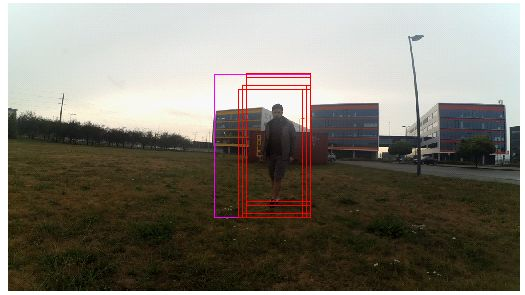
\includegraphics[width=12cm]{3_SVM_model_2_5.jpg}
	\caption{Detekcja na oknie wewnątrz obrazu (skala: 2.5)}
	\label{fig:SVMmodel_2_5}
\end{figure}

\newcolumntype{P}[1]{>{\centering\arraybackslash}p{#1}}
\begin{table}[h]
	\centering
	\caption{Tabela z wynikami dla $5 \times 9$ detekcji z rysunku \ref{fig:SVMmodel_2_5}}
	\begin{tabular}{|P{1.2cm} |P{1.2cm} |P{1.2cm} |P{1.2cm} |P{1.2cm} |P{1.2cm} |P{1.2cm} |P{1.2cm} |P{1.2cm} |}
		
		\hline
    $2.1223$  &  $1.9234$  &  $1.8072$ & $1.8854$  &  $1.6932$ &  $1.5320$  & $ 0.5443$ &  $ 0.2648$  & $\textbf{-0.0366}$ \\ \hline
$1.9547$  &  $2.5649$  &  $1.6400$ & $1.7075$  &  $1.1940$ &  $1.5821$  & $ 0.6492$ &  $ 0.2804$  & $\textbf{-0.0880}$ \\ \hline
$2.5165$  &  $2.7328$  &  $2.3592$ & $2.2650$  &  $2.1196$ &  $1.1509$  & $ 0.8788$ &  $ 0.6314$  & $ 0.1222$ \\ \hline
$2.4744$  &  $2.8618$  &  $2.7310$ & $2.6338$  &  $2.1627$ &  $1.4763$  & $ 0.4520$ &  $\textbf{-0.7166}$  & $\textbf{-1.1757}$ \\ \hline
$2.6806$  &  $2.4200$  &  $2.2032$ & $1.6812$  & $1.9216$ &  $0.9355$  & $\textbf{-0.0505}$ &  $\textbf{-1.3537}$  & $\textbf{-1.3712}$ \\ \hline	
	\end{tabular}
	\label{tab:scale_window_cover_2_5}
\end{table}

\begin{figure}[h]
	\centering
	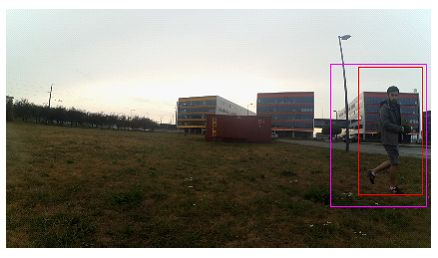
\includegraphics[width=12cm]{3_SVM_model_3.jpg}
	\caption{Detekcja na oknie wewnątrz obrazu (skala: 3)}
	\label{fig:SVMmodel_3}
\end{figure}


\newcolumntype{P}[1]{>{\centering\arraybackslash}p{#1}}
\begin{table}[h]
	\centering
	\caption{Tabela z wynikami dla $5 \times 9$ detekcji z rysunku \ref{fig:SVMmodel_3}}
	\begin{tabular}{|P{1.2cm} |P{1.2cm} |P{1.2cm} |P{1.2cm} |P{1.2cm} |P{1.2cm} |P{1.2cm} |P{1.2cm} |P{1.2cm} |}
	\hline	
    $1.8159$  &  $1.8308$  &  $1.7164$  &  $1.4868$  &  $1.1955$  &  $1.1542$  &  $0.8346$  & $ 0.4625$   & $0.6144$ \\ \hline
$2.3357$  &  $2.6091$  &  $2.0017$  &  $2.0776$  &  $2.2638$  &  $1.8270$  &  $0.6915$  & $\textbf{-0.0323}$  &  $0.6554$ \\ \hline
$2.3233$  &  $2.4182$  &  $1.9292$  &  $2.1127$  &  $1.8924$  &  $1.7307$  &  $0.8044$  & $ 0.3019$  &  $0.7611$ \\ \hline
$1.5705$  &  $1.6276$  &  $1.5120$  &  $1.7848$  &  $1.6619$  &  $1.7323$  &  $0.4511$  & $ 0.8625$  &  $1.1717$ \\ \hline
$1.4874$  &  $1.8153$  &  $1.0768$  &  $1.2884$  &  $1.0186$  &  $1.8310$  &  $0.8986$  & $ 0.6349$  &  $1.1386$ \\ \hline
	\end{tabular}
	\label{tab:scale_window_cover_3}
\end{table}

Następnie wykonano eksperyment pozwalający potwierdzić działanie detekcji dla implementowanych sprzętowo skal: $2/2.5/3/3.5/4$. W tym celu nagrano sekwencję wideo, która przedstawia postać zbliżającą się w stronę kamery z odległości ok. $10$m. W oparciu o nią uruchomiono skrypt realizujący detekcję na wielu skalach, który zaznacza na ramkach obrazu wszystkie obszary zainteresowań oraz najlepsze okno detekcji. Wyniki przedstawia rysunek \ref{fig:SVMmodel_dist}. Dla obu detekcji z pierwszego rzędu, najlepsze wyniki osiągnięto na obszarze w skali równej $2$. Należy zwrócić uwagę, że ze względu na brak uwzględnienia mniejszych skal w teście, na obrazie przeskalowanym ze współczynnikiem $2$ może zostać wykryta osoba o małych rozmiarach względem okna detekcji (przypadek w lewym górnym rogu rysunku). Rzędy drugi oraz trzeci przedstawiają poprawnie wykrytą postać w pozostałych skalach: odpowiednio $2.5/3/3.5/4$. \newline
Eksperyment posłużył również do oszacowania odległości postaci od kamery, które należałoby przyporządkować detekcjom w poszczególnych skalach. Na podstawie minimalnej i maksymalnej odległości osoby od kamery w sekwencji wideo (ok. $2m-10$m) można oszacować, że detekcja w skali $4$ odpowiada odległości ok. $2$m, natomiast każda kolejna skala powiększa tę wartość o ok. $1-1.5$m, aż do odległości ok. $7m$ dla detekcji w skali $2$. Tak jak wspomniano wcześniej, w skali tej wykrywana jest również dalej stojąca osoba (nawet $10$m), choć nie jest to regułą.
\begin{figure}[h]
	\centering
	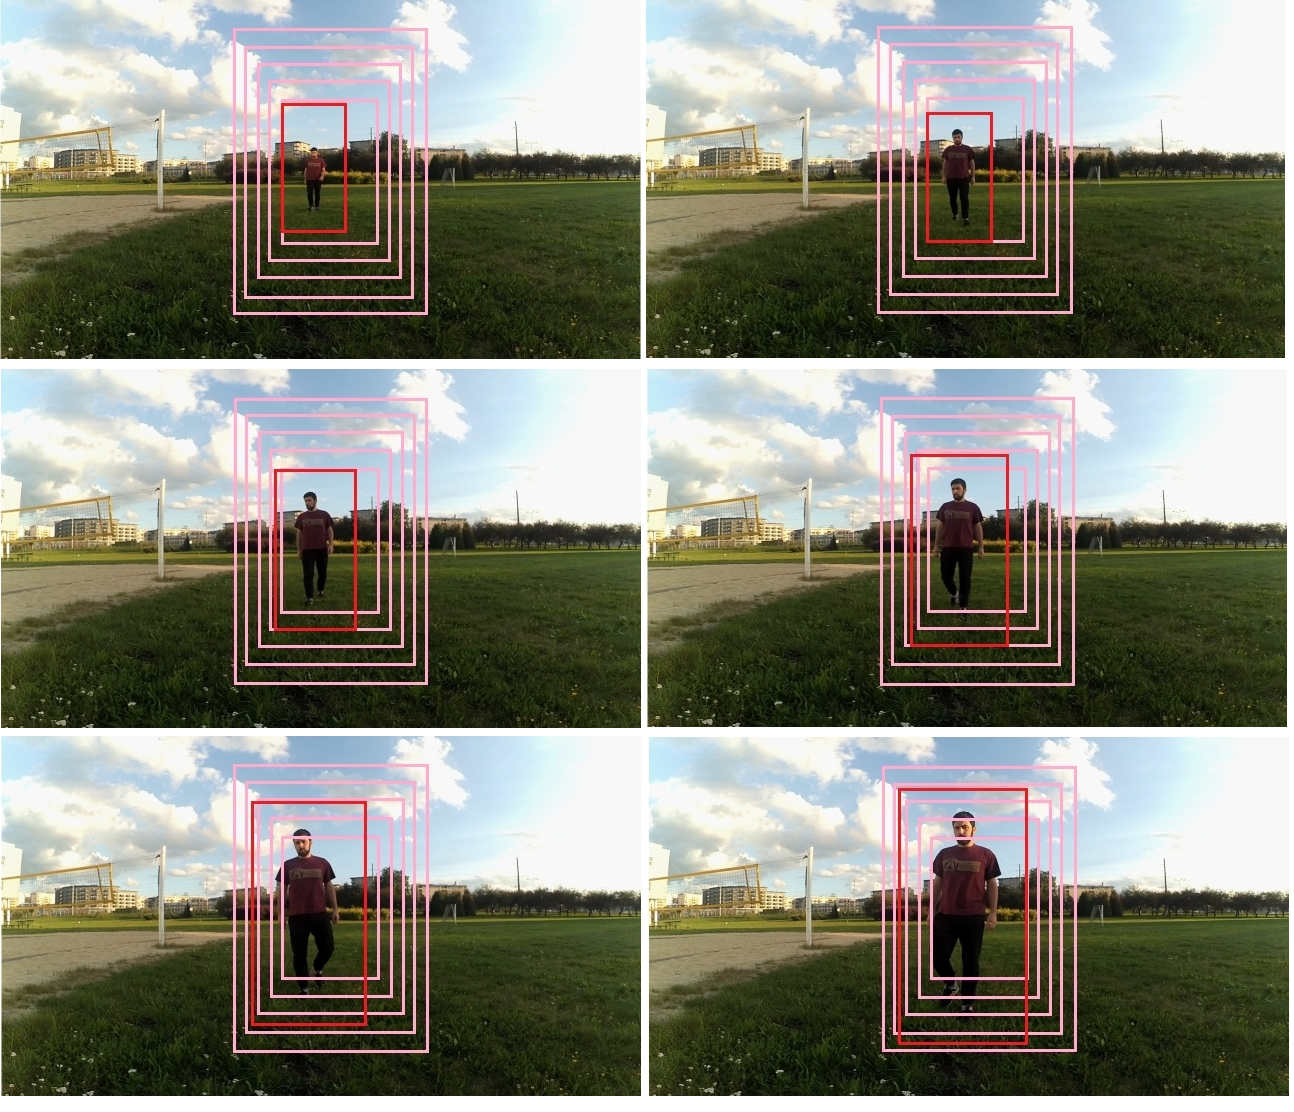
\includegraphics[width=15cm]{HOG_scale_all.jpg}
	\caption{Detekcja dla wielu skal}
	\label{fig:SVMmodel_dist}
\end{figure}

%TODO Czy w jakiś sposób obliczena jest finalna detekcja ? Oraz jak to się przekłada na odległosć. %ODP opisano wyżej jak jest liczona
%TODO Dobrze by było jeszcze zamieścić taki eksperytment - sekwencja na której Pan oddala się od kamery i korespondujące odległości. %ODP Dodano
%TODO Nie wiem czy nie warto rozważyć przetwarzania w więcej niż jednej skali.... albo wszystkich albo przynajmniej sąsiednich (pamiętając tą najlepszą). %ODP Tak robiłem, ale wizualnie to nie ma sensu, bo jest zbyt wiele detekcji i obraz staje się nieczytelny

%TODO BTW, Na takiej sekwencji można też od razu sprawdzić działanie meanshifta. Albo nagrać jeszcze taką gdzie oprócz do przodu idzie się w lewo i prawo... %ODP Nie mam modelu programowego łączącego oba algorytmy, nie wyrobiłem czasowo żeby go połączyć